%% LyX 1.6.7 created this file.  For more info, see http://www.lyx.org/.
%% Do not edit unless you really know what you are doing.
\documentclass[english,msc]{ubcthesis}
\usepackage[T1]{fontenc}
\usepackage[latin9]{inputenc}
\usepackage{longtable}
\usepackage{url}
\usepackage{graphicx}
\usepackage{esint}
\usepackage[numbers]{natbib}

\makeatletter

%%%%%%%%%%%%%%%%%%%%%%%%%%%%%% LyX specific LaTeX commands.
%% Because html converters don't know tabularnewline
\providecommand{\tabularnewline}{\\}

%%%%%%%%%%%%%%%%%%%%%%%%%%%%%% User specified LaTeX commands.
%%
%% This is file `ubcsample.tex',
%% generated with the docstrip utility.
%
% The original source files were:
%
% ubcthesis.dtx  (with options: `ubcsampletex')
%% 
%% This file was generated from the ubcthesis package.
%% --------------------------------------------------------------
%% 
%% Copyright (C) 2001
%% Michael McNeil Forbes
%% mforbes@alum.mit.edu
%% 
%% This file may be distributed and/or modified under the
%% conditions of the LaTeX Project Public License, either version 1.2
%% of this license or (at your option) any later version.
%% The latest version of this license is in
%%    http://www.latex-project.org/lppl.txt
%% and version 1.2 or later is part of all distributions of LaTeX
%% version 1999/12/01 or later.
%% 
%% This program is distributed in the hope that it will be useful,
%% but WITHOUT ANY WARRANTY; without even the implied warranty of
%% MERCHANTABILITY or FITNESS FOR A PARTICULAR PURPOSE.  See the
%% LaTeX Project Public License for more details.
%% 
%% This program consists of the files ubcthesis.dtx, ubcthesis.ins, and
%% the sample figures fig.eps and fig.fig.
%% 
%% This file may be modified and used as a base for your thesis without
%% including the licence agreement as long as the content (i.e. textual
%% body) of the file is completely rewritten. You must, however, change
%% the name of the file.
%% 
%% This file may only be distributed together with a copy of this
%% program. You may, however, distribute this program without generated
%% files such as this one.
%% 

% This Sample thesis requires \LaTeX2e
\NeedsTeXFormat{LaTeX2e}[1995/12/01]
\ProvidesFile{ubcsample.tex}[2010/06/13 v1.66 ^^J
 University of British Columbia Sample Thesis]
% This is the \documentclass[]{} command.  The manditory argument
% specifies the "flavour" of thesis (ubcthesis for UBC).  The
% optional arguments (in []) specify options that affect how the
% thesis is displayed.  Please see the ubcthesis documentation for
% details about the options.

%
% To compile this sample thesis, issue the following commands:
% latex ubcsample
% bibtex ubcsample
% latex ubcsample
% latex ubcsample
% latex ubcsample
%
% To view use xdvi (on unix systems):
% xdvi ubcsample.dvi
%
% To make a postscript file, use dvips:
% dvips -o ubcsample.ps ubcsample.dvi
%
% To view the postscript file, use ghostview or gv (on unix systems):
% gv ubcsample.ps
%
%************************************************
% Optional packages.
%
% The use of these packages is optional, but they provide various
% tools for more flexible formating.  The sample thesis uses these,
% but if you remove the example code, you should be able to exclude
% these packages.  Only standard packages have been described here;
% they should be installed with any complete LaTeX instalation, but
% if not, you can find them at the Comprehensive TeX Archive Network
% (CTAN): http://www.ctan.org/
%

%******** afterpage ***************************
% This package allows you to issue commands at the end of the current
% page.  A good use for this is to use the command
% \afterpage{\clearpage} right after a figure.  This will cause the
% figure to be inserted on the page following the current one (or on
% the current page if it will fit) but will not break the page in the
% middle.
\usepackage{afterpage}

%******** float *********************************
% This package allows you to customize the style of
% "floats"---floating objects such as figures and tables.  In
% addition, it allows you to define additional floating objects which
% may be included in a list similar to that produces by \listoftables
% and \listoffigures.  Common uses include introducing floats for
% programs and other code bits in Compute Science and Chemical Schema.
\usepackage{float}

%******** tocloft *******************************
% This package allows you to customize and define custom lists such
% as a list of programs or Chemical Scheme.  Note: if you use the
% subfigure package, you must specify that you do as an option here.
% The title option uses the default formatting.  We do not use this
% here as the default formatting is acceptable.  Use the float
% package instead unless you need the extra formatting control
% provided by tocloft.
%\usepackage[subfigure, titles]{tocloft}

%******** alltt *********************************
% The alltt package allows you to include files and have them
% formatted in a verbatim fashion.  This is useful for including
% source code from an additional file.
%\usepackage{alltt}

%******** listings ******************************
% The listings package may be used to include chunks of source code
% and has facilities for pretty-printing many languages.
%\usepackage{listings}

%******** longtable *****************************
% The longtable package allows you to define tables that span
% multiple pages.
\usepackage{longtable}

%******** graphics and graphicx *****************
% This allows you to include encapsulated postscript files.  If you
% don't have this, comment the \includegraphics{} line following the
% comment "%includegraphics" later in this file.


%******** subfigure *****************************
% The subfigure package allows you to include multiple figures and
% captions within a single figure environment.
%\usepackage{subfigure}

%******** here **********************************
% The here package gives you more control over the placement of
% figures and tables.  In particular, you can specify the placement
% "H" which means "Put the figure here" rather than [h] which means
% "I would suggest that you put the figure here if you think it looks
% good."
%\usepackage{here}

%******** pdflscape ********************************
% This allows you to include landscape layout pages by using the
% |landscape| environment.  The use of |pdflscape| is preferred over
% the standard |lscape| package because it automatically rotates the
% page in the pdf file for easier reading.  (Thanks to Joseph Shea
% for pointing this out.)
\usepackage{pdflscape}

%******** natbib ********************************
% This is a very nice package for bibliographies.  It includes options
% for sorting and compressing bibliographic entries.


%******** psfrag ******************************
% This allows you to replace text in postscript pictures with formated
% latex text.  This allows you to use math in graph labels
% etc. Uncomment the psfrag lines following the "%psfrag" comment
% later in this file if you don't have this package.  The replacements
% will only be visible in the final postscript file: they will be
% listed in the .dvi file but not performed.
\usepackage{psfrag}

%******** hyperref *****************************
% Please read the manual:
% http://www.tug.org/applications/hyperref/manual.html
%
% This adds hyperlinks to your document: with the right viewers (later
% versions of xdvi, acrobat with pdftex, latex2html etc.) this will
% make your equation, figure, citation references etc. hyperlinks so
% that you can click on them.  Also, your table of contents will be
% able to take you to the appropriate sections.  In the viewers that
% support this, the links often appear with an underscore.  This
% underscore will not appear in printed versions.
%
% Note: if you do not use the hypertex option, then the dvips driver
% may be loaded by default.  This will cause the entries in the list
% of figures and list of tables to be on a single line because dvips
% does not deal with hyperlinks on broken lines properly.
%
% NOTE: HYPERREF is sensitive to the ORDER in which it is LOADED.
% For example, it must be loaded AFTER natbib but BEFORE newly
% defined float environments.  See the README file with the hyperref
% for some help with this.  If you have some very obscure errors, try
% first disabling hyperref.  If that fixes the problem, try various
% orderings.
%
% Note also that there is a bug with versions before 2003/11/30
% v6.74m that cause the float package to not function correctly.
% Please ensure you have a current version of this package.  A
% warning will be issued if you leave the date below but do not have
% a current version installed.
%
% Some notes on options: depending on how you build your files, you
% may need to choose the appropriate option (such as [pdftex]) for the
% backend driver (see the hyperref manual for a complete list).  Also,
% the default here is to make links from the page numbers in the table
% of contents and lists of figures etc.  There are other options:
% excluding the [linktocpage] option will make the entire text a
% hyperref, but for some backends will prevent the text from wrapping
% which can look terrible.  There is a [breaklinks=true] option that
% will be set if the backend supports (dvipdfm for example supports
% it but does not work with psfrag.)
%
% Finally, there are many options for choosing the colours of the
% links.  These will be included by default in future versions but
% you should probably consider changing some now for the electronic
% version of your thesis.
\usepackage[unicode=true,
  linktocpage,
  linkbordercolor={0.5 0.5 1},
  citebordercolor={0.5 1 0.5},
  linkcolor=blue]{hyperref}

% If you would like to compile this sample thesis without the
% hyperref package, then you will need to comment out the previous
% \usepackage command and uncomment the following command which will
% put the URL's in a typewriter font but not link them.
%\newcommand\url[1]{\texttt{#1}}

%******** setspace *******************************
% The setspace package allows you to manually set the spacing of the
% file.  UBC may require 1.5 spacing for microfilming of theses.  In
% this case you may obtain this by including this package and issuing
% one of the following commands:
%\usepackage{setspace}
%\singlespacing
%\onehalfspacing
%\doublespacing

% These commands are optional.  The defaults are shown.  You only
% need to include them if you need a different value
\institution{The University Of British Columbia}

% If you are at the Okanagan campus, then you should specify these
% instead.
%\faculty{The College of Graduate Studies}
%\institutionaddress{Okanagan}
\faculty{The Faculty of Graduate Studies}
\institutionaddress{Vancouver}

% You can issue as many of these as you have...
\previousdegree{B.Sc., The University of British Columbia, 1999}
\previousdegree{M.Sc., The University of British Columbia, 2001}
\previousdegree{Ph.D., Massachusetts Institute of Technology, 2005}

% You can override the option setting here.
% \degreetitle{Jack of All Trades}

% These commands are required.
\title{A Sample UBC Thesis}
\subtitle{With a Subtitle}
\author{Michael M$^{\rm c}$Neil Forbes}
\copyrightyear{2000}
\submitdate{\today} % The "\ " is required after
                                      % \monthname to prevent the
                                      % command from eating the space.
\program{Physics}

% These commands are presently not required for UBC theses as the
% advisor's name and title are not presently required anywhere.
%\advisor{Ariel R.~Zhitnitsky}
%\advisortitle{Professor of Physics}

% One might want to override the format of the section and chapter
% numbers.  This shows you how to do it.  Note that the current
% format is acceptable for submission to the FoGS: If you wish to modify
% these, you should check with the FoGS explicity. prior to making
% the modifications.
\renewcommand{\thepart}{\Roman{part}}
\renewcommand{\thechapter}{\arabic{chapter}}
\renewcommand{\thesection}{\thechapter.\arabic{section}}
\renewcommand{\thesubsection}{\thesection.\arabic{subsection}}
\renewcommand{\thesubsubsection}{\thesubsection.\arabic{subsubsection}}
\renewcommand{\theparagraph}{\thesubsubsection.\arabic{paragraph}}
\renewcommand{\thesubparagraph}{\theparagraph.\arabic{subparagraph}}




% Here is an example of a "Program" environment defined with the
% "float" package.  The list of programs will be stored in the file
% ubcsample.lop and the numbering will start with the chapter
% number.  The style will be "ruled".
\floatstyle{ruled}
\newfloat{Program}{htbp}{lop}[chapter]

% Here is the start of the document.


\makeatother

\usepackage{babel}

\begin{document}
% This starts numbering in Roman numerals as required for the thesis
% style.
\frontmatter % Mandatory


% The order of the following components should be preserved.  The order
% listed here is the order currently required by FoGS.
% Mandatory
% Mandatory -  maximum 350 words

\begin{abstract}
The \texttt{genthesis.cls} \LaTeX{} class file and accompanying documents,
such as this sample thesis, are distributed in the hope that it will
be useful but without any warranty (without even the implied warranty
of fitness for a particular purpose). For a description of this file's
purpose, and instructions on its use, see below.

These files are distributed under the GPL which should be included
here in the future. Please let the author know of any changes or improvements
that should be made.

Michael Forbes. mforbes@physics.ubc.ca 
\end{abstract}
\tableofcontents{}% Mandatory
\listoftables
% Mandatory if thesis has tables
\listoffigures
% Mandatory if thesis has figures
\listof{Program}{List of Programs} % Optional
% Any other lists should come here, i.e.
% Abbreviation schemes, definitions, lists of formulae, list of
% schemes, glossary, list of symbols etc.



\chapter{Acknowledgements}

% Optional
This is the place to thank professional colleagues and people who
have given you the most help during the course of your graduate work.


\chapter{Dedication}

% Optional
The dedication is usually quite short, and is a personal rather than
an academic recognition. The \emph{Dedication} does not have to be
titled, but it must appear in the table of contents. If you want to
skip the chapter title but still enter it into the Table of Contents,
use this command \verb|\chapter[Dedication]{}|.


\chapter{Statement of Co-Authorship}

% Manditory if thesis co-written
If any part of your thesis was co-written, you must include a Co-Authorship
statement which gives details of your contribution to the following
areas:
\begin{itemize}
\item identification and design of research program 
\item performing the research 
\item data analyses 
\item manuscript preparation 
\end{itemize}
Note that this section is the last of the preliminary pages (with
lowercase Roman numeral page numbers). It must be placed \emph{before}
the \verb|\mainmatter| command. After that, Arabic numbered pages
will begin.

% Any other unusual prefactory material should come here before the
% main body.


% Now regular page numbering begins.
\mainmatter

% Parts are the largest structural units, but are optional.
%\part{Thesis}


% Chapters are the next main unit.



\chapter{This is a Chapter}

% Sections are a sub-unit



\section{A Section}

Here is a section with some text. Equations look like this $y=x$.%
\footnote{Here is a footnote.%
}

This is an example of a second paragraph in a section so you can see
how much it is indented by.

% Subsections follow



\subsection{This is a Subsection}

Here is an example of a citation: \citep{Forbes:2006ba}. The actual
form of the citation is governed by the bibliographystyle. These citations
are maintained in a BIB\TeX{} file \texttt{sample.bib}. You could
type these directly into the file. For an example of the format to
use look at the file \texttt{ubcsample.bbl} after you compile this
file.%
\footnote{Here is another footnote.%
}

This is an example of a second paragraph in a subsection so you can
see how much it is indented by.


\subsubsection{This is a Subsubsection}

Here are some more citations \citep{LL3:1977,Peccei:1989,Turner:1999}.
If you use the \texttt{natbib} package with the \verb+sort&compress+
option, then the following citation will look the same as the first
citation in this section: \citep{Turner:1999,Peccei:1989,LL3:1977}.

This is an example of a second paragraph in a subsubsection so you
can see how much it is indented by.


\paragraph{This is a Paragraph}

Paragraphs and subparagraphs are the smallest units of text. There
is no subsubsubsection etc.


\subparagraph{This is a Subparagraph}

This is the last level of organisation. If you need more than this,
you should consider reorganizing your work\dots

\begin{equation}
\mathrm{f}(x)=\int_{-\infty}^{\int_{-\infty}^{x}e^{-\frac{y^{2}}{2}}\mathrm{d}{y}}e^{-z^{2}}\mathrm{d}z\end{equation}


In order to show you what a separate page would look like (i.e. without
a chapter heading) I must type some more text. Thus I will babble
a bit and keep babbling for at least one more page\ldots{} What you
should notice is that the chapter titles appear substantially lower
than the continuing text. Babble babble babble babble babble babble
babble babble babble babble babble babble babble babble babble babble
babble babble babble babble babble babble babble babble babble babble
babble babble babble babble babble babble babble babble babble babble
babble babble babble babble babble.

Babble babble babble babble babble babble babble babble babble babble
babble babble babble babble babble babble babble babble babble babble
babble babble babble babble babble babble babble babble babble babble
babble babble babble babble babble babble babble babble babble babble
babble babble babble babble babble babble babble babble babble babble
babble babble babble babble babble babble babble babble babble babble
babble babble babble babble babble babble babble babble babble babble
babble babble babble babble babble babble babble babble babble babble
babble babble babble babble babble babble babble babble babble babble
babble babble babble babble babble babble babble babble babble babble
babble babble babble babble babble babble babble babble babble babble
babble babble babble babble babble babble babble babble babble babble
babble babble babble babble.

%
\begin{table}[t]
 %optional [t, b or h];
 \begin{tabular}{|r||r@{.}l}
\hline 
Phoenix  & \$960 & 35\tabularnewline
\hline 
Calgary  & \$250 & 00\tabularnewline
\hline
\end{tabular}\caption[Here is the caption for this wonderful table\ldots{}]{ \label{tab:Table1} Here is the caption for this wonderful table.
It has not been centered and the positioning has been specified to
be at the top of the page. Thus it appears above the babble rather
than below where it is defined in the source file.}

\end{table}


% Force a new page: without this, the quote would appear on the
% previous page.
\newpage{}


\section{Quote}

% It is centered

\begin{quote}
\begin{center}
This is a small poem,\\
 a little poem, a Haiku,\\
 to show you how to.\\
 ---Michael M$^{{\rm c}}$Neil Forbes. 
\par\end{center}
\end{quote}
This small poem shows several features: 
\begin{itemize}
\item The use of the \verb|quote| and \verb|center| environments. 
\item The \verb|\newpage| command has been used to force a page break.
(Sections do not usually start on a new page.) 
\item The pagestyle has been set to suppress the headers using the command
\verb|\thispagestyle{plain}|. Note that using \verb|\pagestyle{plain}|
would have affected all of the subsequent pages. 
\end{itemize}

\section{Programs}

Here we give an example of a new float as defined using the \texttt{float}
package. In the preamble we have use the commands \begin{verbatim}
\floatstyle{ruled} \newfloat{Program}{htbp}{lop}{[}chapter{]}
\end{verbatim} This creates a {}``Program'' environment that may
be use for program fragments. A sample \texttt{python} program is
show as Program~\ref{prog:fib}. (Note that Python places a fairly
restrictive limit on recursion so trying to call this with a large
$n$ before building up the cache is likely to fail unless you increase
the recursion depth.) \begin{Program} \caption{\label{prog:fib} Python program that computes the $n^{{\rm th}}$
Fibonacci number using memoization.}


\begin{verbatim} def fib(n,cache={}): if n < 2: return 1 if n in
cache: return cache{[}n{]} else: result = fib(n-1)+fib(n-2) cache{[}n{]}
= result return result \end{verbatim} \end{Program} Instead of using
a \texttt{verbatim} environment for your program chunks, you might
like to \texttt{include} them within an \texttt{alltt} envrironment
by including the \verb|\usepackage{alltt}| package (see page 187
of the \LaTeX{} book). Another useful package is the \verb|\usepackage{listings}|
which can pretty-print many different types of source code.

% Force a new page
\newpage{}

% Here we provide a short optional argument to \chapter[]{}.  This
% optional argument will appear in the table of contents.  For long
% titles, one should use this to give a single-line entry to the
% table of contents.



\chapter[Another Chapter\ldots{}]{Another Chapter with a Very Long Chapter-name that will Probably
Cause Problems}

This chapter name is very long and does not display properly in the
running headers or in the table of contents. To deal with this, we
provide a shorter version of the title as the optional argument to
the \verb|\chapter[]{}| command.

For example, this chapter's title and associated table of contents
heading and running header was created with\\
 \verb|\chapter[Another Chapter\ldots]{Another Chapter with a Very Long|\\
 \verb|Chapter-name that will Probably Cause Problems}|.

Note that, according to the thesis regulations, the heading included
in the table of contents must be a truncation of the actual heading. 


\section{Another Section}

Another bunch of text to demonstrate what this file does. You might
want a list for example:%
\footnote{Here is a footnote in a different chapter. Footnotes should come after
punctuation.%
} 
\begin{itemize}
\item An item in a list. 
\item Another item in a list. 
\end{itemize}

\section*{An Unnumbered Section That is Not Included in the Table of Contents}

Here is an example of a figure environment. %
\begin{figure}[ht]
 %psfrag: comment the following line if not using the psfrag package


\centering{}\psfrag{pie makes me happy!}{$\pi$ makes me happy!}
%includegraphics: comment the following if not using the graphicx package
 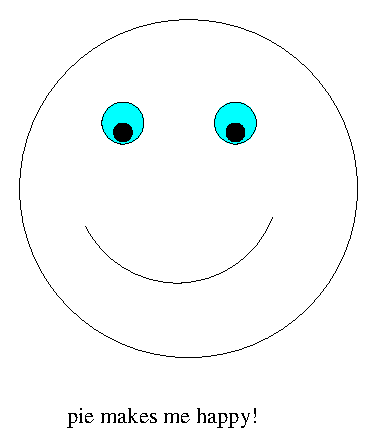
\includegraphics[width=0.4\textwidth]{fig} \caption[Happy Face: figure example.]{\label{fig:happy} This is a figure of a happy face with a \texttt{psfrag}
replacement. The original figure (drawn in xfig and exported to a
.eps file) has the text {}``pie makes me happy!''. The \texttt{psfrag}
package replaces this with {}``$\pi$ makes me happy!''. Note that
we have used the optional argument for the caption command so that
only a short version of this caption occurs in the list of figures.}

\end{figure}


\afterpage{\clearpage{}} Perhaps I should say that the example
of a figure can be seen in Figure~\ref{fig:happy}. Figure placement
can be tricky with \LaTeX{}\ because figures and tables are treated
as {}``floats'': text can flow around them, but if there is not
enough space, they will appear later. To prevent figures from going
too far, the \verb|\afterpage{\clearpage}| command can be used. This
makes sure that the figure appears on the following page.

The \verb|\clearpage| forces a page break so that the figure can
be placed, but without the the \verb|\afterpage{}| command, the page
would be broken too early (at the \verb|\clearpage| statement). The
\verb|\afterpage{}| command tells \LaTeX{} to issue the command after
the present page has been rendered.

Figures can make a document more enjoyable as demonstrated by Figure~\ref{fig:happy}.


\section{Tables}

We have already included one table:~\ref{tab:Table1}. Another table
is plopped right here. %
\begin{table}[ht]
 

\centering{}\begin{tabular}{|l||l|l||l|l|}
\hline 
 & \multicolumn{2}{l|}{Singular} & \multicolumn{2}{l|}{Plural}\tabularnewline
\hline 
 & English & \textbf{Gaeilge} & English & \textbf{Gaeilge}\tabularnewline
\hline
\hline 
1st Person & at me & \textbf{agam} & at us & \textbf{againn}\tabularnewline
2nd Person & at you & \textbf{agat} & at you & \textbf{agaibh}\tabularnewline
3rd Person & at him & \textbf{aige} & at them & \textbf{acu}\tabularnewline
 & at her & \textbf{aici} &  & \tabularnewline
\hline
\end{tabular}\caption{ \label{tab:Table2} Another table.}

\end{table}


Well, actually, as with Figure~\ref{fig:happy}, the table does not
necessarily appear right {}``here'' because tables are also {}``floats''.
\LaTeX{} puts them where it can. Becuase of this, one should refer
to floats by their labels rather than by their location. This example
is demonstrated by Table~\ref{tab:Table2}. This one is pretty close,
however.

Another useful package is \verb|\usepackage{longtable}| which provides
the \texttt{longtable} environment. This is nice because it allows
tables to span multiple pages. Table~\ref{tab:longtable} has been
formatted this way. 

\begin{center}
\begin{longtable}{|l|l|l|}
\caption{\label{tab:longtable}Feasible triples for highly variable Grid}
\tabularnewline
\caption{\label{tab:longtable}Feasible triples for highly variable Grid}
\tabularnewline
\hline 
\multicolumn{1}{|c|}{\textbf{Time (s)}} & \multicolumn{1}{c|}{\textbf{Triple chosen}} & \multicolumn{1}{c|}{\textbf{Other feasible triples}}\tabularnewline
\endfirsthead
\hline 
\multicolumn{3}{c}{}\tabularnewline
\hline 
\multicolumn{1}{|c|}{\textbf{Time (s)}} & \multicolumn{1}{c|}{\textbf{Triple chosen}} & \multicolumn{1}{c|}{\textbf{Other feasible triples}}\tabularnewline
\hline
\endhead
\hline 
\multicolumn{3}{|r|}{{Continued on next page}}\tabularnewline
\hline
\endfoot
\hline 
0  & (1, 11, 13725)  & (1, 12, 10980), (1, 13, 8235), (2, 2, 0), (3, 1, 0) \tabularnewline
274  & (1, 12, 10980)  & (1, 13, 8235), (2, 2, 0), (2, 3, 0), (3, 1, 0) \tabularnewline
5490  & (1, 12, 13725)  & (2, 2, 2745), (2, 3, 0), (3, 1, 0) \tabularnewline
8235  & (1, 12, 16470)  & (1, 13, 13725), (2, 2, 2745), (2, 3, 0), (3, 1, 0) \tabularnewline
10980  & (1, 12, 16470)  & (1, 13, 13725), (2, 2, 2745), (2, 3, 0), (3, 1, 0) \tabularnewline
13725  & (1, 12, 16470)  & (1, 13, 13725), (2, 2, 2745), (2, 3, 0), (3, 1, 0) \tabularnewline
16470  & (1, 13, 16470)  & (2, 2, 2745), (2, 3, 0), (3, 1, 0) \tabularnewline
19215  & (1, 12, 16470)  & (1, 13, 13725), (2, 2, 2745), (2, 3, 0), (3, 1, 0) \tabularnewline
21960  & (1, 12, 16470)  & (1, 13, 13725), (2, 2, 2745), (2, 3, 0), (3, 1, 0) \tabularnewline
24705  & (1, 12, 16470)  & (1, 13, 13725), (2, 2, 2745), (2, 3, 0), (3, 1, 0) \tabularnewline
27450  & (1, 12, 16470)  & (1, 13, 13725), (2, 2, 2745), (2, 3, 0), (3, 1, 0) \tabularnewline
30195  & (2, 2, 2745)  & (2, 3, 0), (3, 1, 0) \tabularnewline
32940  & (1, 13, 16470)  & (2, 2, 2745), (2, 3, 0), (3, 1, 0) \tabularnewline
35685  & (1, 13, 13725)  & (2, 2, 2745), (2, 3, 0), (3, 1, 0) \tabularnewline
38430  & (1, 13, 10980)  & (2, 2, 2745), (2, 3, 0), (3, 1, 0) \tabularnewline
41175  & (1, 12, 13725)  & (1, 13, 10980), (2, 2, 2745), (2, 3, 0), (3, 1, 0) \tabularnewline
43920  & (1, 13, 10980)  & (2, 2, 2745), (2, 3, 0), (3, 1, 0) \tabularnewline
46665  & (2, 2, 2745)  & (2, 3, 0), (3, 1, 0) \tabularnewline
49410  & (2, 2, 2745)  & (2, 3, 0), (3, 1, 0) \tabularnewline
52155  & (1, 12, 16470)  & (1, 13, 13725), (2, 2, 2745), (2, 3, 0), (3, 1, 0) \tabularnewline
54900  & (1, 13, 13725)  & (2, 2, 2745), (2, 3, 0), (3, 1, 0) \tabularnewline
57645  & (1, 13, 13725)  & (2, 2, 2745), (2, 3, 0), (3, 1, 0) \tabularnewline
60390  & (1, 12, 13725)  & (2, 2, 2745), (2, 3, 0), (3, 1, 0) \tabularnewline
63135  & (1, 13, 16470)  & (2, 2, 2745), (2, 3, 0), (3, 1, 0) \tabularnewline
65880  & (1, 13, 16470)  & (2, 2, 2745), (2, 3, 0), (3, 1, 0) \tabularnewline
68625  & (2, 2, 2745)  & (2, 3, 0), (3, 1, 0) \tabularnewline
71370  & (1, 13, 13725)  & (2, 2, 2745), (2, 3, 0), (3, 1, 0) \tabularnewline
74115  & (1, 12, 13725)  & (2, 2, 2745), (2, 3, 0), (3, 1, 0) \tabularnewline
76860  & (1, 13, 13725)  & (2, 2, 2745), (2, 3, 0), (3, 1, 0) \tabularnewline
79605  & (1, 13, 13725)  & (2, 2, 2745), (2, 3, 0), (3, 1, 0) \tabularnewline
82350  & (1, 12, 13725)  & (2, 2, 2745), (2, 3, 0), (3, 1, 0) \tabularnewline
85095  & (1, 12, 13725)  & (1, 13, 10980), (2, 2, 2745), (2, 3, 0), (3, 1, 0) \tabularnewline
87840  & (1, 13, 16470)  & (2, 2, 2745), (2, 3, 0), (3, 1, 0) \tabularnewline
90585  & (1, 13, 16470)  & (2, 2, 2745), (2, 3, 0), (3, 1, 0) \tabularnewline
93330  & (1, 13, 13725)  & (2, 2, 2745), (2, 3, 0), (3, 1, 0) \tabularnewline
96075  & (1, 13, 16470)  & (2, 2, 2745), (2, 3, 0), (3, 1, 0) \tabularnewline
98820  & (1, 13, 16470)  & (2, 2, 2745), (2, 3, 0), (3, 1, 0) \tabularnewline
101565  & (1, 13, 13725)  & (2, 2, 2745), (2, 3, 0), (3, 1, 0) \tabularnewline
104310  & (1, 13, 16470)  & (2, 2, 2745), (2, 3, 0), (3, 1, 0) \tabularnewline
107055  & (1, 13, 13725)  & (2, 2, 2745), (2, 3, 0), (3, 1, 0) \tabularnewline
109800  & (1, 13, 13725)  & (2, 2, 2745), (2, 3, 0), (3, 1, 0) \tabularnewline
112545  & (1, 12, 16470)  & (1, 13, 13725), (2, 2, 2745), (2, 3, 0), (3, 1, 0) \tabularnewline
115290  & (1, 13, 16470)  & (2, 2, 2745), (2, 3, 0), (3, 1, 0) \tabularnewline
118035  & (1, 13, 13725)  & (2, 2, 2745), (2, 3, 0), (3, 1, 0) \tabularnewline
120780  & (1, 13, 16470)  & (2, 2, 2745), (2, 3, 0), (3, 1, 0) \tabularnewline
123525  & (1, 13, 13725)  & (2, 2, 2745), (2, 3, 0), (3, 1, 0) \tabularnewline
126270  & (1, 12, 16470)  & (1, 13, 13725), (2, 2, 2745), (2, 3, 0), (3, 1, 0) \tabularnewline
129015  & (2, 2, 2745)  & (2, 3, 0), (3, 1, 0) \tabularnewline
131760  & (2, 2, 2745)  & (2, 3, 0), (3, 1, 0) \tabularnewline
134505  & (1, 13, 16470)  & (2, 2, 2745), (2, 3, 0), (3, 1, 0) \tabularnewline
137250  & (1, 13, 13725)  & (2, 2, 2745), (2, 3, 0), (3, 1, 0) \tabularnewline
139995  & (2, 2, 2745)  & (2, 3, 0), (3, 1, 0) \tabularnewline
142740  & (2, 2, 2745)  & (2, 3, 0), (3, 1, 0) \tabularnewline
145485  & (1, 12, 16470)  & (1, 13, 13725), (2, 2, 2745), (2, 3, 0), (3, 1, 0) \tabularnewline
148230  & (2, 2, 2745)  & (2, 3, 0), (3, 1, 0) \tabularnewline
150975  & (1, 13, 16470)  & (2, 2, 2745), (2, 3, 0), (3, 1, 0) \tabularnewline
153720  & (1, 12, 13725)  & (2, 2, 2745), (2, 3, 0), (3, 1, 0) \tabularnewline
156465  & (1, 13, 13725)  & (2, 2, 2745), (2, 3, 0), (3, 1, 0) \tabularnewline
159210  & (1, 13, 13725)  & (2, 2, 2745), (2, 3, 0), (3, 1, 0) \tabularnewline
161955  & (1, 13, 16470)  & (2, 2, 2745), (2, 3, 0), (3, 1, 0) \tabularnewline
164700  & (1, 13, 13725)  & (2, 2, 2745), (2, 3, 0), (3, 1, 0) \tabularnewline
\end{longtable}
\par\end{center}


\subsection*{An Unnumbered Subsection}

Note that if you use subsections or further divisions under an unnumbered
section, then you should make them unnumbered as well otherwise you
will end up with zeros in the section numbering.


\chapter{Landscape Mode}

The landscape mode allows you to rotate a page through 90 degrees.
It is generally not a good idea to make the chapter heading landscape,
but it can be useful for long tables etc.

\begin{landscape} This text should appear rotated, allowing for formatting
of very wide tables etc. Note that this might only work after you
convert the \texttt{dvi} file to a postscript (\texttt{ps}) or \texttt{pdf}
file using \texttt{dvips} or \texttt{dvipdf} etc. This features is
provided by the \verb|lscape| and the \verb|pdflscape| packages.
The latter is preferred if it works as it also rotates the pages in
the pdf file for easier viewing. \end{landscape}

% This file is setup to use a bibtex file sample.bib and uses the
% plain style.  Other styles may be used depending on the conventions
% of your field of study.
% Note: the bibliography must come before the appendices.
\bibliographystyle{plain} \bibliographystyle{plain}
\bibliography{sample}


% Use this to reset the appendix counter.  Note that the FoGS
% requires that the word ``Appendices'' appear in the table of
% contents either before each appendix lable or as a division
% denoting the start of the appendices.  We take the latter option
% here.  This is ensured by making the \texttt{appendicestoc} option
% a default option to the UBC thesis class.


% If you only have one appendix, please uncomment the following line.


\appendix
%dummy comment inserted by tex2lyx to ensure that this paragraph is not empty



\chapter{First Appendix}

Here you can have your appendices. Note that if you only have a single
appendix, you should issue \verb|\renewcommand{\appendicesname}{Appendix}|
before calling \verb|\appendix| to display the singular {}``Appendix''
rather than the default plural {}``Appendices'' some


\chapter{Second Appendix}

Here is the second appendix.

% Indices come here.



\chapter*{Additional Information}

This chapter shows you how to include additional information in your
thesis, the removal of which will not affect the submission. Such
material should be removed before the thesis is actually submitted.

First, the chapter is unnumbered and not included in the Table of
Contents. Second, it is the last section of the thesis, so its removal
will not alter any of the page numbering etc. for the previous sections.
Do not include any floats, however, as these will appear in the initial
lists.

The \texttt{ubcthesis} \LaTeX{} class has been designed to aid you
in producing a thesis that conforms to the requirements of The University
of British Columbia Faculty of Graduate Studies (FoGS).

Proper use of this class and sample is highly recommended---and should
produce a well formatted document that meets the FoGS requirement.
Notwithstanding, complex theses may require additional formatting
that may conflict with some of the requirements. We therefore \emph{highly
recommend} that you consult one of the FoGS staff for assistance and
an assessment of potential problems \emph{before} starting final draft.

While we have attemped to address most of the thesis formatting requirements
in these files, they do not constitute an official set of thesis requirements.
The official requirements are available at the following section of
the FoGS web site: 

\begin{center}
\begin{tabular}{|l|}
\hline 
\url{http://www.grad.ubc.ca/students/thesis/}\tabularnewline
\hline
\end{tabular}
\par\end{center}

We recommend that you review these instructions carefully.
\end{document}
